\documentclass{article}

%################################# Preliminar
% Symbols
\usepackage[T1]{fontenc}
\usepackage{upgreek}
\usepackage{physics}
\usepackage{cancel}
\usepackage{amsfonts, amsthm}
\usepackage{amssymb, latexsym, amsmath}
\usepackage{ textcomp }

% Proof
\renewcommand*{\proofname}{\textbf{Demostra\'on:}}

% Theorem
\newtheorem*{theorem}{Teorema}

%Algorithms
\usepackage[ruled,lined,linesnumbered,commentsnumbered]{algorithm2e}

%% Identación
\setlength{\parindent}{0cm}

% Código
\newcommand{\code}[1]{\textcolor{white!25!black}{\texttt{#1}}}
\usepackage{listings}

%AMS
\usepackage{amsthm}
\newtheorem{algo-thm}{Algoritmo}

% Graphics
\usepackage{graphicx}
\usepackage{pgf}

% Margins
\addtolength{\voffset}{-1.5cm}
\addtolength{\hoffset}{-1.5cm}
\addtolength{\textwidth}{3cm}
\addtolength{\textheight}{3cm}

% Color a letras.
%\usepackage[usenames,dvipsnames,svgnames,table]{xcolor}

% Tikz
\usepackage{tkz-graph}
\usepackage{tikz}
\usetikzlibrary{arrows,automata}
\usepackage{tikz}
\usetikzlibrary{arrows,automata}
%\usetikzlibrary[topaths]

% Def. Dr. César.
\usetikzlibrary{shapes,calc}
\tikzstyle{edge}=[shorten <=2pt, shorten >=2pt, >=stealth, line width=1.1pt]
\tikzstyle{blueE}=[shorten <=2pt, shorten >=2pt, >=stealth, line width=1.5pt, blue]
\tikzstyle{blackV}=[circle, fill=black, minimum size=6pt, inner sep=0pt, outer sep=0pt]
\tikzstyle{blueV}=[circle, fill=blue, draw, minimum size=6pt, line width=0.75pt, inner sep=0pt, outer sep=0pt]
\tikzstyle{redV}=[circle, fill=red, draw, minimum size=6pt, line width=0.75pt, inner sep=0pt, outer sep=0pt]
\tikzstyle{redSV}=[semicircle, fill=red, minimum size=3pt, inner sep=0pt, outer sep=0pt, rotate=225]
\tikzstyle{blueSV}=[semicircle, fill=blue, minimum size=3pt, inner sep=0pt, outer sep=0pt, rotate=225]
\tikzstyle{blackSV}=[semicircle, fill=black, minimum size=3pt, inner sep=0pt, outer sep=0pt, rotate=225]
\tikzstyle{vertex}=[circle, draw, minimum size=6pt, line width=0.75pt, inner sep=0pt, outer sep=0pt]

%\pagenumbering{gobble} -- Este comando
%                       -- quita el número de página.

%Header-Footer
\usepackage{fancyhdr}
\renewcommand{\headrulewidth}{1pt}

\newcommand{\set}[1]{
  \left\{ #1 \right\}
}

\footskip = 50pt
\renewcommand{\headrulewidth}{1pt}

\pagestyle{fancyplain}

%################################# Inicio de documento
\begin{document}
	\title{UNIVERSIDAD NACIONAL AUT\'ONOMA DE M\'EXICO\\ Facultad de Ciencias}
\author{ Adri\'an Aguilera Moreno   - 421005200 }
\date{}
\maketitle
\begin{center}
  
\includegraphics[scale=0.20]{../Portada/Portada}\\[0.4cm]
  \Large
  \bf{Seminario de Computación B: Estructuras de Datos Avanzadas.}
  \normalsize
\end{center}
\newpage
\fancyhead[r]{ Seminario de Computación B: Estructuras de Datos Avanzadas 2024-1}


	\section*{\LARGE{Tarea 01}}

        \textbf{\textcolor{blue}{1.}} Tienes la siguiente sucesión elementos $S = \{5,17,6,8,2,4,1,12,10,3,21\}$. Toma los elementos de dicha sucesión únicamente de izquierda a derecha para los siguientes ejercicios, es decir, el primer elemento a extraer será el $5$, luego el $17$, el $6$, etc... (4 puntos)

\begin{enumerate}

    \item Inserta los 5 primeros elementos dentro de una pila. Saca dos veces el elemento al tope de la pila. Mete los siguientes 4 elementos de $S$. Saca otros 2 elementos de la pila. Por último, ingresa un elemento más. Si sacas todos los elementos de la pila restantes, ¿En qué orden salen? (0.5 pts.)

    \item Inserta los 6 primeros elementos dentro de una cola. Saca 4 elementos de la cola. Ingresa todos los elementos restantes de $S$. Saca otros 3 elementos. Si sacas todos los elementos de la cola restantes, ¿En qué orden salen? (0.5 pts.)
    
    \item Construye un árbol binario ordenado con los elementos de $S$ insertándolos conforme éstos son dados (Ojo, no necesitas balancear el árbol). (0.5 pts.)

    \item Dado el árbol anterior. Realiza una rotación en el nodo que contiene al 17 hacia la derecha. (0.5 pts.)

    \item Ahora sobre el árbol resultante anterior. Realiza una rotación en el nodo que contiene al 6 hacia la izquierda. (0.5 pts.)

    \item Realiza un recorrido BFS sobre el árbol resultante anterior. ¿En qué orden son devueltos los elementos? (0.5 pts.)

    \item Realiza 2 recorridos DFS sobre el árbol resultante del ejercicio 5, uno en pre-orden y otro en post-orden. ¿En qué orden son devueltos los elementos en cada caso? (1 pts.)

\end{enumerate}

$\rhd$\textbf{Solución.}
    \begin{enumerate}
    \item Insertar los 5 primeros elementos dentro de una pila
       \begin{center}
          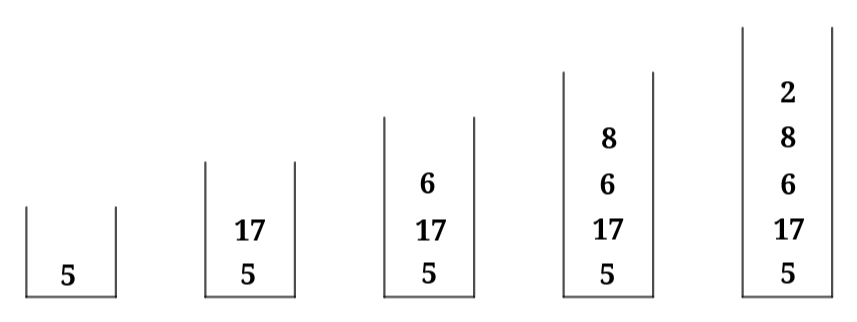
\includegraphics[scale=0.3]{../Image/P1.png}
       \end{center}
       Sacar dos veces el elemento al tope de la pila
       \begin{center}
          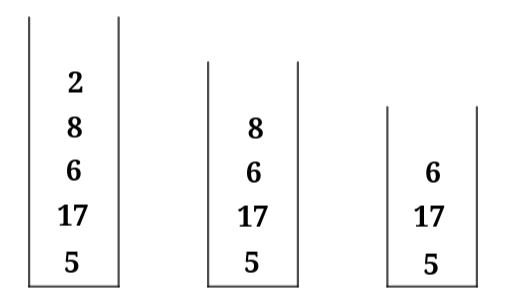
\includegraphics[scale=0.3]{../Image/P2.png}
       \end{center}
       Meter los siguientes 4 elementos de $S$
       \begin{center}
          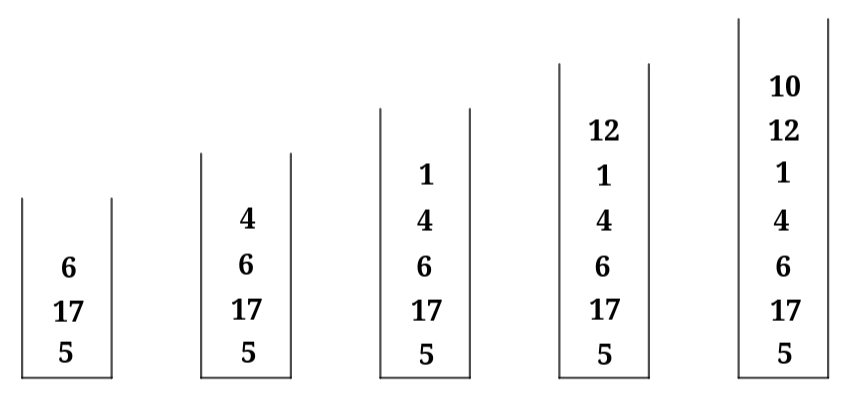
\includegraphics[scale=0.3]{../Image/P3.png}
       \end{center}
       Sacar otros 2 elementos de la pila
       \begin{center}
          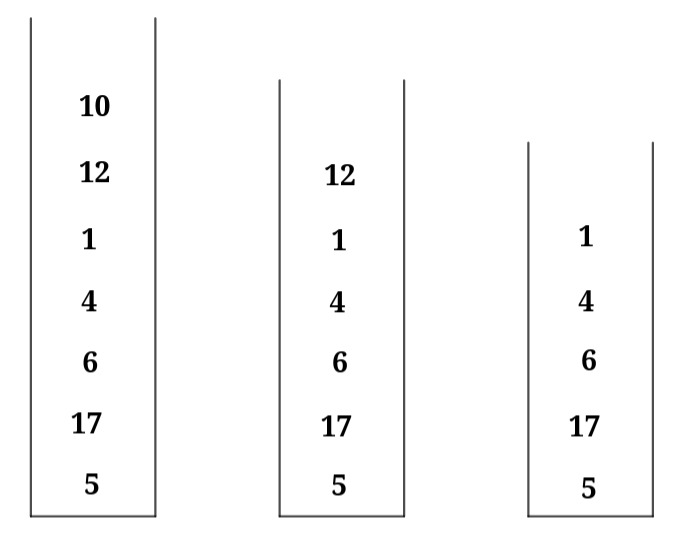
\includegraphics[scale=0.3]{../Image/P4.png}
       \end{center}
       ingresa un elemento más
       \begin{center}
          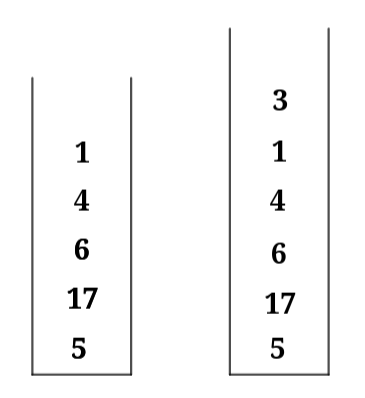
\includegraphics[scale=0.3]{../Image/P5.png}
       \end{center}
       ¿En qué orden salen? [3, 1, 4, 6, 17, 5].
       
       \item Insertar los 6 primeros elementos dentro de una cola
       \begin{center}
          
\includegraphics[scale=0.3]{../Image/C1.png}
       \end{center}
       Sacar 4 elementos de la cola
       \begin{center}
          
\includegraphics[scale=0.3]{../Image/C2.png}
       \end{center}
       Ingresar todos los elementos restantes de $S$
       \begin{center}
          
\includegraphics[scale=0.3]{../Image/C3.png}
       \end{center}
       Sacar otros 3 elementos
       \begin{center}
          
\includegraphics[scale=0.3]{../Image/C4.png}
       \end{center}
       Si sacas todos los elementos de la cola restantes, ¿En qué orden salen? [12, 10, 3, 21].
       \item Construye un árbol binario ordenado con los elementos de $S$ insertándolos conforme
       éstos son dados
       \begin{center}
          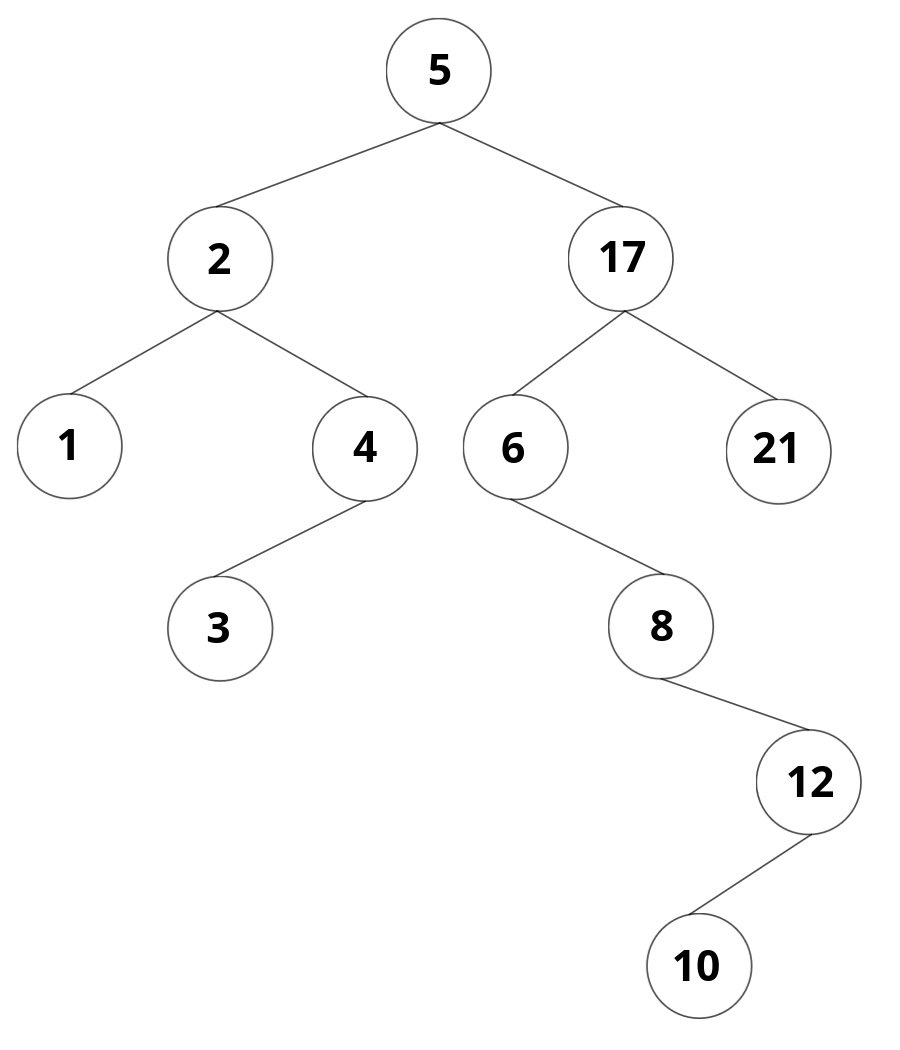
\includegraphics[scale=0.19]{../Image/BST.png}
       \end{center}
       \item Dado el árbol anterior. Realiza una rotación en el nodo que contiene al 17 hacia la derecha
       \begin{center}
          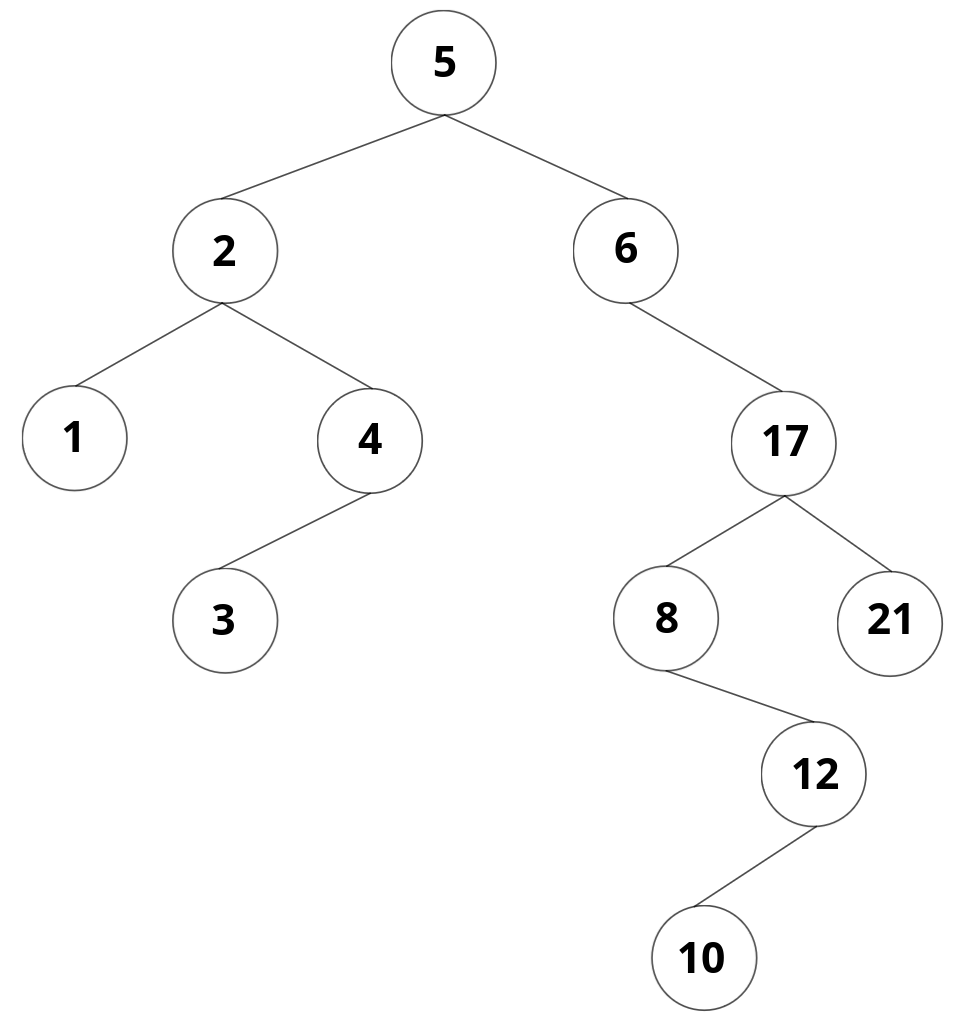
\includegraphics[scale=0.19]{../Image/RD.png}
       \end{center}
       \item Ahora sobre el árbol resultante anterior. Realiza una rotación en el nodo que contiene
       al 6 hacia la izquierda
       \begin{center}
          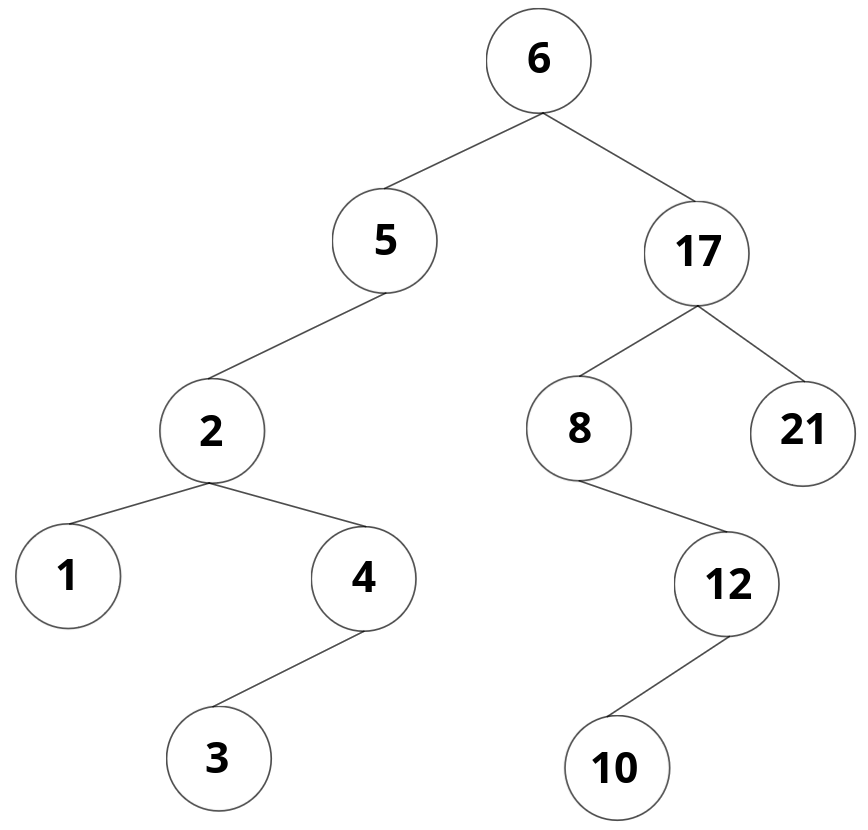
\includegraphics[scale=0.19]{../Image/RI.png}
       \end{center}
       \item Realiza un recorrido BFS sobre el árbol resultante anterior.
       ¿En qué orden son devueltos los elementos? [6, 5, 17, 2, 8, 21, 1, 4, 12, 3, 10].
       \item Realiza 2 recorridos DFS sobre el árbol resultante del ejercicio 5,
       uno en pre-orden y otro en post-orden. ¿En qué orden son devueltos los elementos en cada caso?
       \newcommand{\localtextbulletone}{\textcolor{gray}{\raisebox{.45ex}{\rule{.6ex}{.6ex}}}}
       \renewcommand{\labelitemi}{\localtextbulletone}
       \begin{itemize}
       \item pre-orden: [6, 5, 2, 1, 4, 3, 17, 8, 12, 10, 21].
       \item post-orden: [1, 3, 4, 2, 5, 10, 12, 8, 21, 17, 6].
       \end{itemize}
    \end{enumerate}

\hfill $\lhd$
\newline
        
        \textbf{\textcolor{blue}{2.}} Tenemos dos árboles binarios de búsqueda con O(n) elementos cada uno y queremos construir una lista de tamaño O(2n)  con los elementos de ambos árboles de tal manera que la lista resultante este ordenada de mayor a menor. Diseña un algoritmo de complejidad O(n) para obtener esta lista, justifica la complejidad y explica claramente tu algoritmo con un ejemplo. Nota: Toma en cuenta que el árbol binario de búsqueda puede tener elementos repetidos. (2 puntos)\newline


$\rhd$\textbf{Solución.} El algoritmo solicitado es el siguiente: para 2 pilas $p_1$ y $p_2$,
con una lista $l$.
\begin{enumerate}
\item De nuestros dos árboles, digamos $T_1$ y $T_2$, recorramos ambos con \textit{DFS in-order}
  y guardemoslos valores devueltos en las pilas $p_1$ y $p_2$ respectivamente para cada árbol.\newline

  \textbf{Obs.} Cómo $T_1$ y $T_2$ son \textit{BST}, entonces el recorrido \textit{DFS in-order}
  nos regresa sus valores en orden ascendente desde el fondo de la pila al tope.
\item Sacamos los valores de la pila de manera paralela, siempre insertando el tope mayor de
  sus respectivas pilas a $l$. Si los topes, digamos $t_1$ y $t_2$, son iguales es indistinto e
  insertamos ambos a $l$. Si una de las dos pilas termina sus elementos, entonces vaciamos la
  restante y vamos insertando sus elementos en $l$.
\end{enumerate}
\textit{Análisis de complejidad.} A continuación se detalla el análisis de tiempo:
\begin{enumerate}
\item Recorrer una gráfica mediante DFS es del orden de $\mathcal{O}(|V| + |E|)$, en este caso
  partícular recorremos dos árboles y por tanto su complejidad es del orden de sus nodos, por lo cuál
  tenemos una complejidad contenida en $\mathcal{O}(\cdot|V_{T_1}| + \cdot|V_{T_2}|) = \mathcal{O}(2\cdot|V|) = \mathcal{O}(n)$. Nuevamente, insertar los elementos en las respectivas pilas es una operación del
  orden de $\mathcal{O}(n)$.
\item Sacar los elementos de las pilas e insertarlos a $l$ nos cuesta $\mathcal{O}(2n) = \mathcal{O}(n)$.
  Pues basta sacar los elementos de la pila e insertar en $l$ (dos operaciones por elemento).
\end{enumerate}
Así, concluimos que nuestra complejidad está contenida en
\[\mathcal{O}(n) + \mathcal{O}(n) = \mathcal{O}(n).\]
\hfill $\lhd$
\newline
        
        \textbf{\textcolor{blue}{3.}} Preparata se encuentra haciendo el programa "X", el programa "X" es un juego para resolver un cubo Rubik, el usuario analiza el estado de  un cubo Rubik en tres dimensiones y con base en su criterio  elije una de las operaciones $a_1 ... a_n$, para modificar el estado del cubo, Preparata sabe que estas operaciones tienen "inversa" es decir si la operación $a_1$ nos lleva del estado $e_1$ al estado $e_2$ entonces la inversa de la operación $a_1$ nos regresa al estado $e_1$, el ya tiene programadas todas las operaciones con sus respectivas operaciones inversas, pero no sabe como implementar la transición y el regreso de los estados para que el usuario pueda hacer una operación o deshacerla, el usuario también puede realizar varias operaciones y deshacerlas todas o una parte de ellas, además si ya deshizo un conjunto de operaciones puede volver a recrearlas sin necesidad de volver a pensar en ellas.
    
El cree que una estructura de datos le podría ayudar con esto. Ayudale a Preparata a descubrir la estructura de datos que necesita y explica detalladamente como  implementar la transición y el regreso de los estados, la complejidad de tu solución debe ser de orden $O(1)$ para deshacer una operación o para recrearla. Nota: Las operaciones tienen orden. (2 puntos)\newline

$\rhd$\textbf{Solución.} Para este problema podemos hacer uso de $2$ pilas cómo estructura
de datos para el almacenamiento de las operaciones aplicadas ¿De qué manera?
\begin{enumerate}
\item En la pila, digamos $P_1$, insertamos las operaciones. Sin en algún momento requerimos
  \textit{deshacer} la operación más reciente sacamos el tope de la pila. Si requerimos regresarnos
  $i$-operaciones, entonces sacamos $i$ topes de $P_1$ y regresamos al estado partícular que
  queremos.
\item ¿Cómo hacemos que tenga memoria? Los elementos que saquemos de $P_1$ los ingresamos a la
  segunda pila, digamos $P_2$, si en algún momento necesitamos recordar la operación que deshicimos
  basta consultar el tope de $P_2$.
\end{enumerate}
\textit{Análisis de complejidad.} A continuación se desglosa la complejidad de operaciones:
\begin{enumerate}
\item Insertar en la pila nos cuesta $\mathcal{O}(1)$.
\item Sacar el tope de la pila nos cuesta $\mathcal{O}(1)$.
\end{enumerate}
En total, nuestra complejidad es del orden $\mathcal{O}(1)$ por \textit{deshacer} o \textit{rehacer}
una operación.
\hfill $\lhd$
\newpage

        \textbf{\textcolor{blue}{4.}} Urrutia esta trabajando en un nuevo proyecto para obtener cuentas de detalle de tablas de información, por ejemplo tenemos las siguientes dos tablas:

\begin{center}
    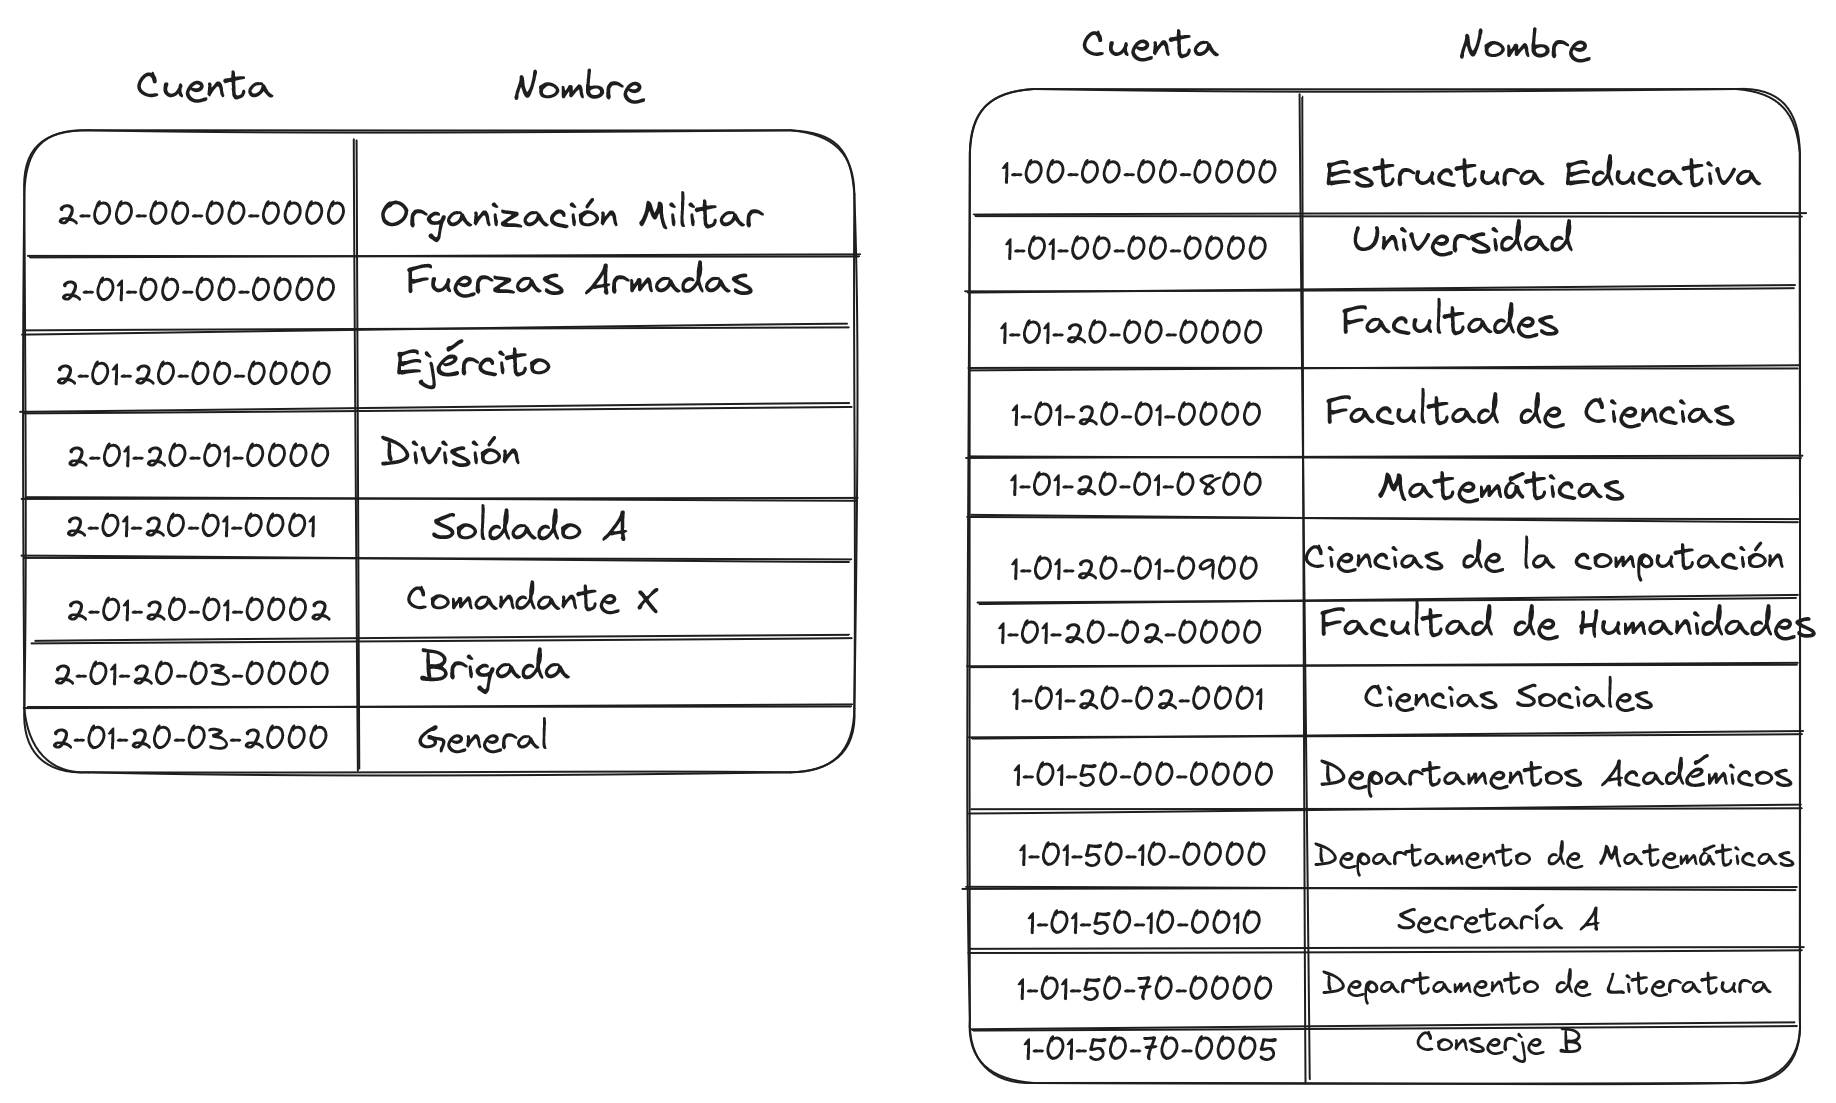
\includegraphics[scale=0.2]{../Image/Tablas.png}
\end{center}
    
Estas tablas contiene información ordenada de formar jerárquica, y a nosotros nos interesaa extraer la información de menor jerarquía pero sin perder el nombre de las cuentas de mayor jerarquía a las que pertenecen, es decir buscamos una tabla como resultado final de esta manera:

\begin{center}
    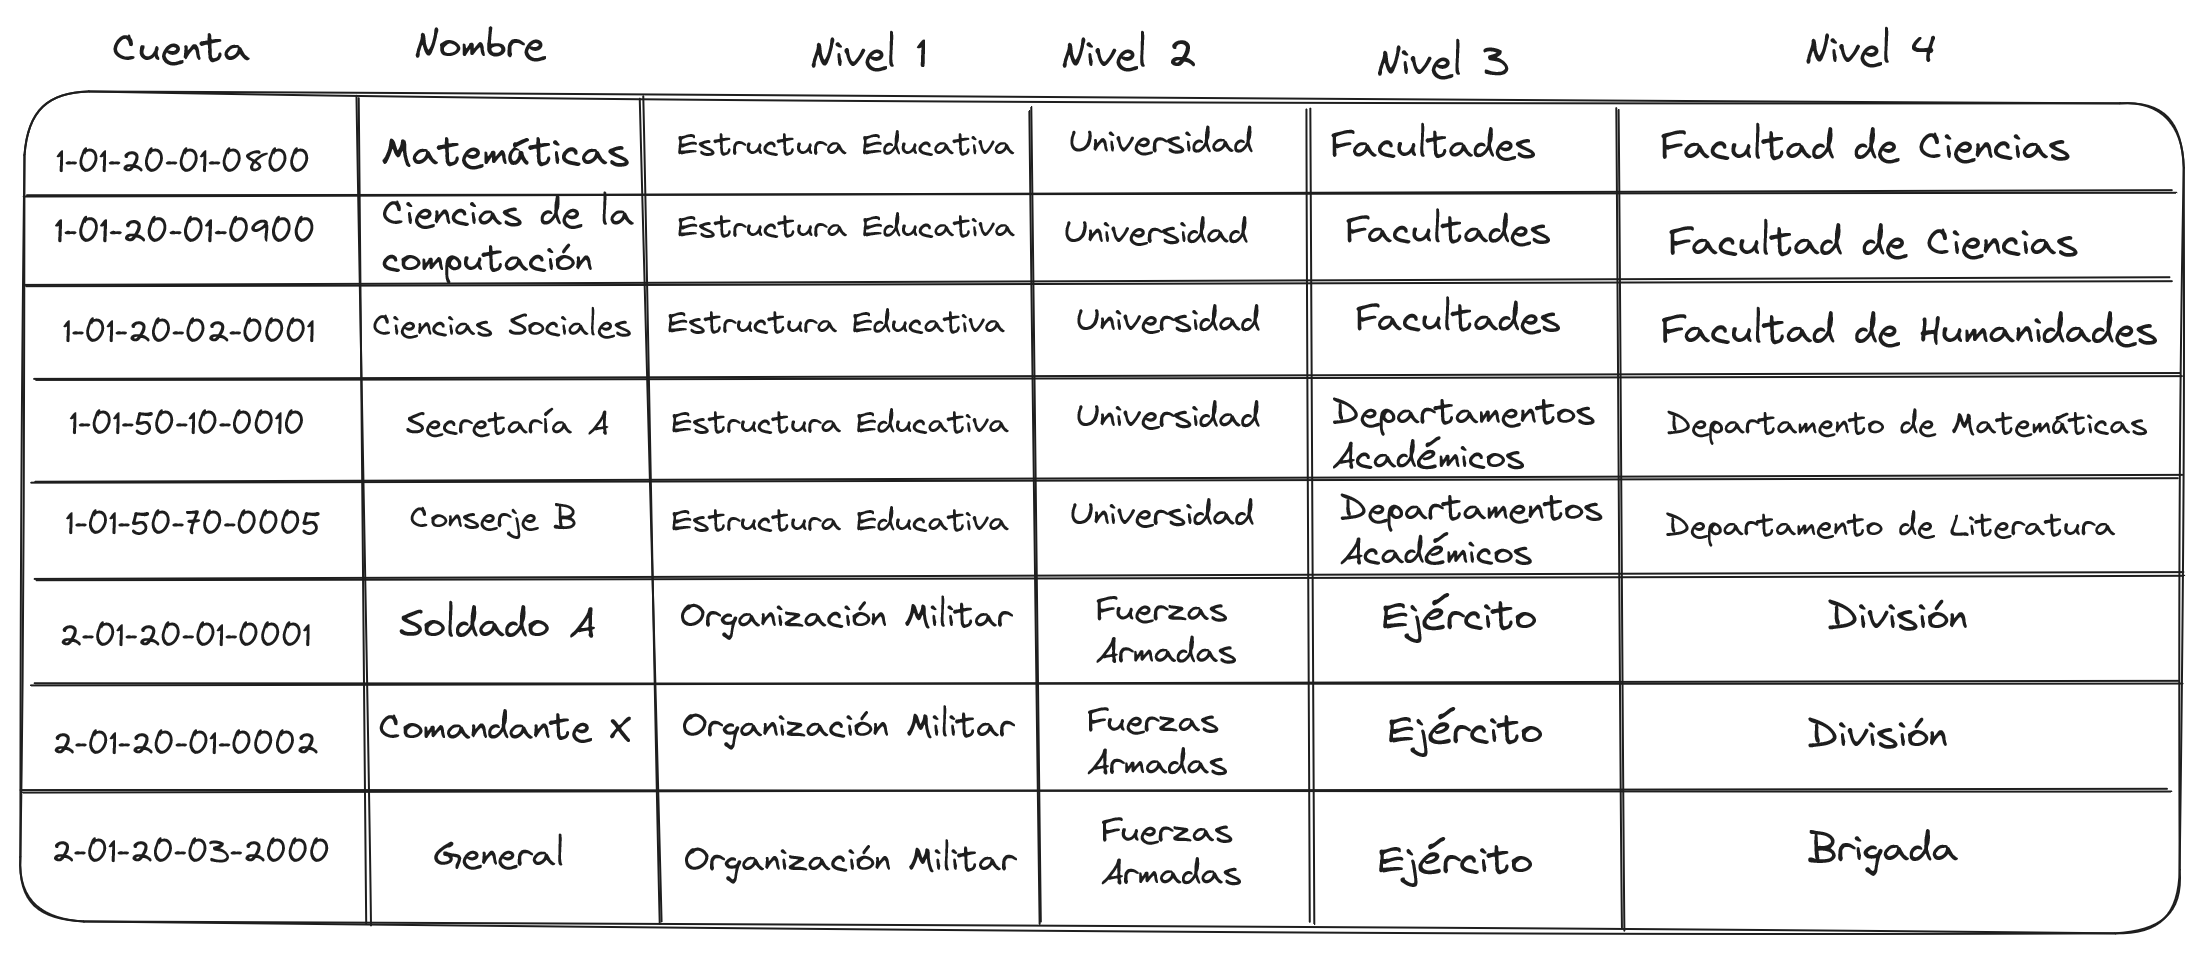
\includegraphics[scale=0.2]{../Image/Resultado.png}
\end{center}

Urrutia se dio cuenta que puede construir un árbol n-ario para resolver de manera fácil este problema basándose en los números de cuenta para construir una llave que le ayudará a decidir si un nodo es hijo o no de otro nodo, hizo un diagrama que representa como debería quedar su árbol n-ario:
\newpage

\begin{center}
    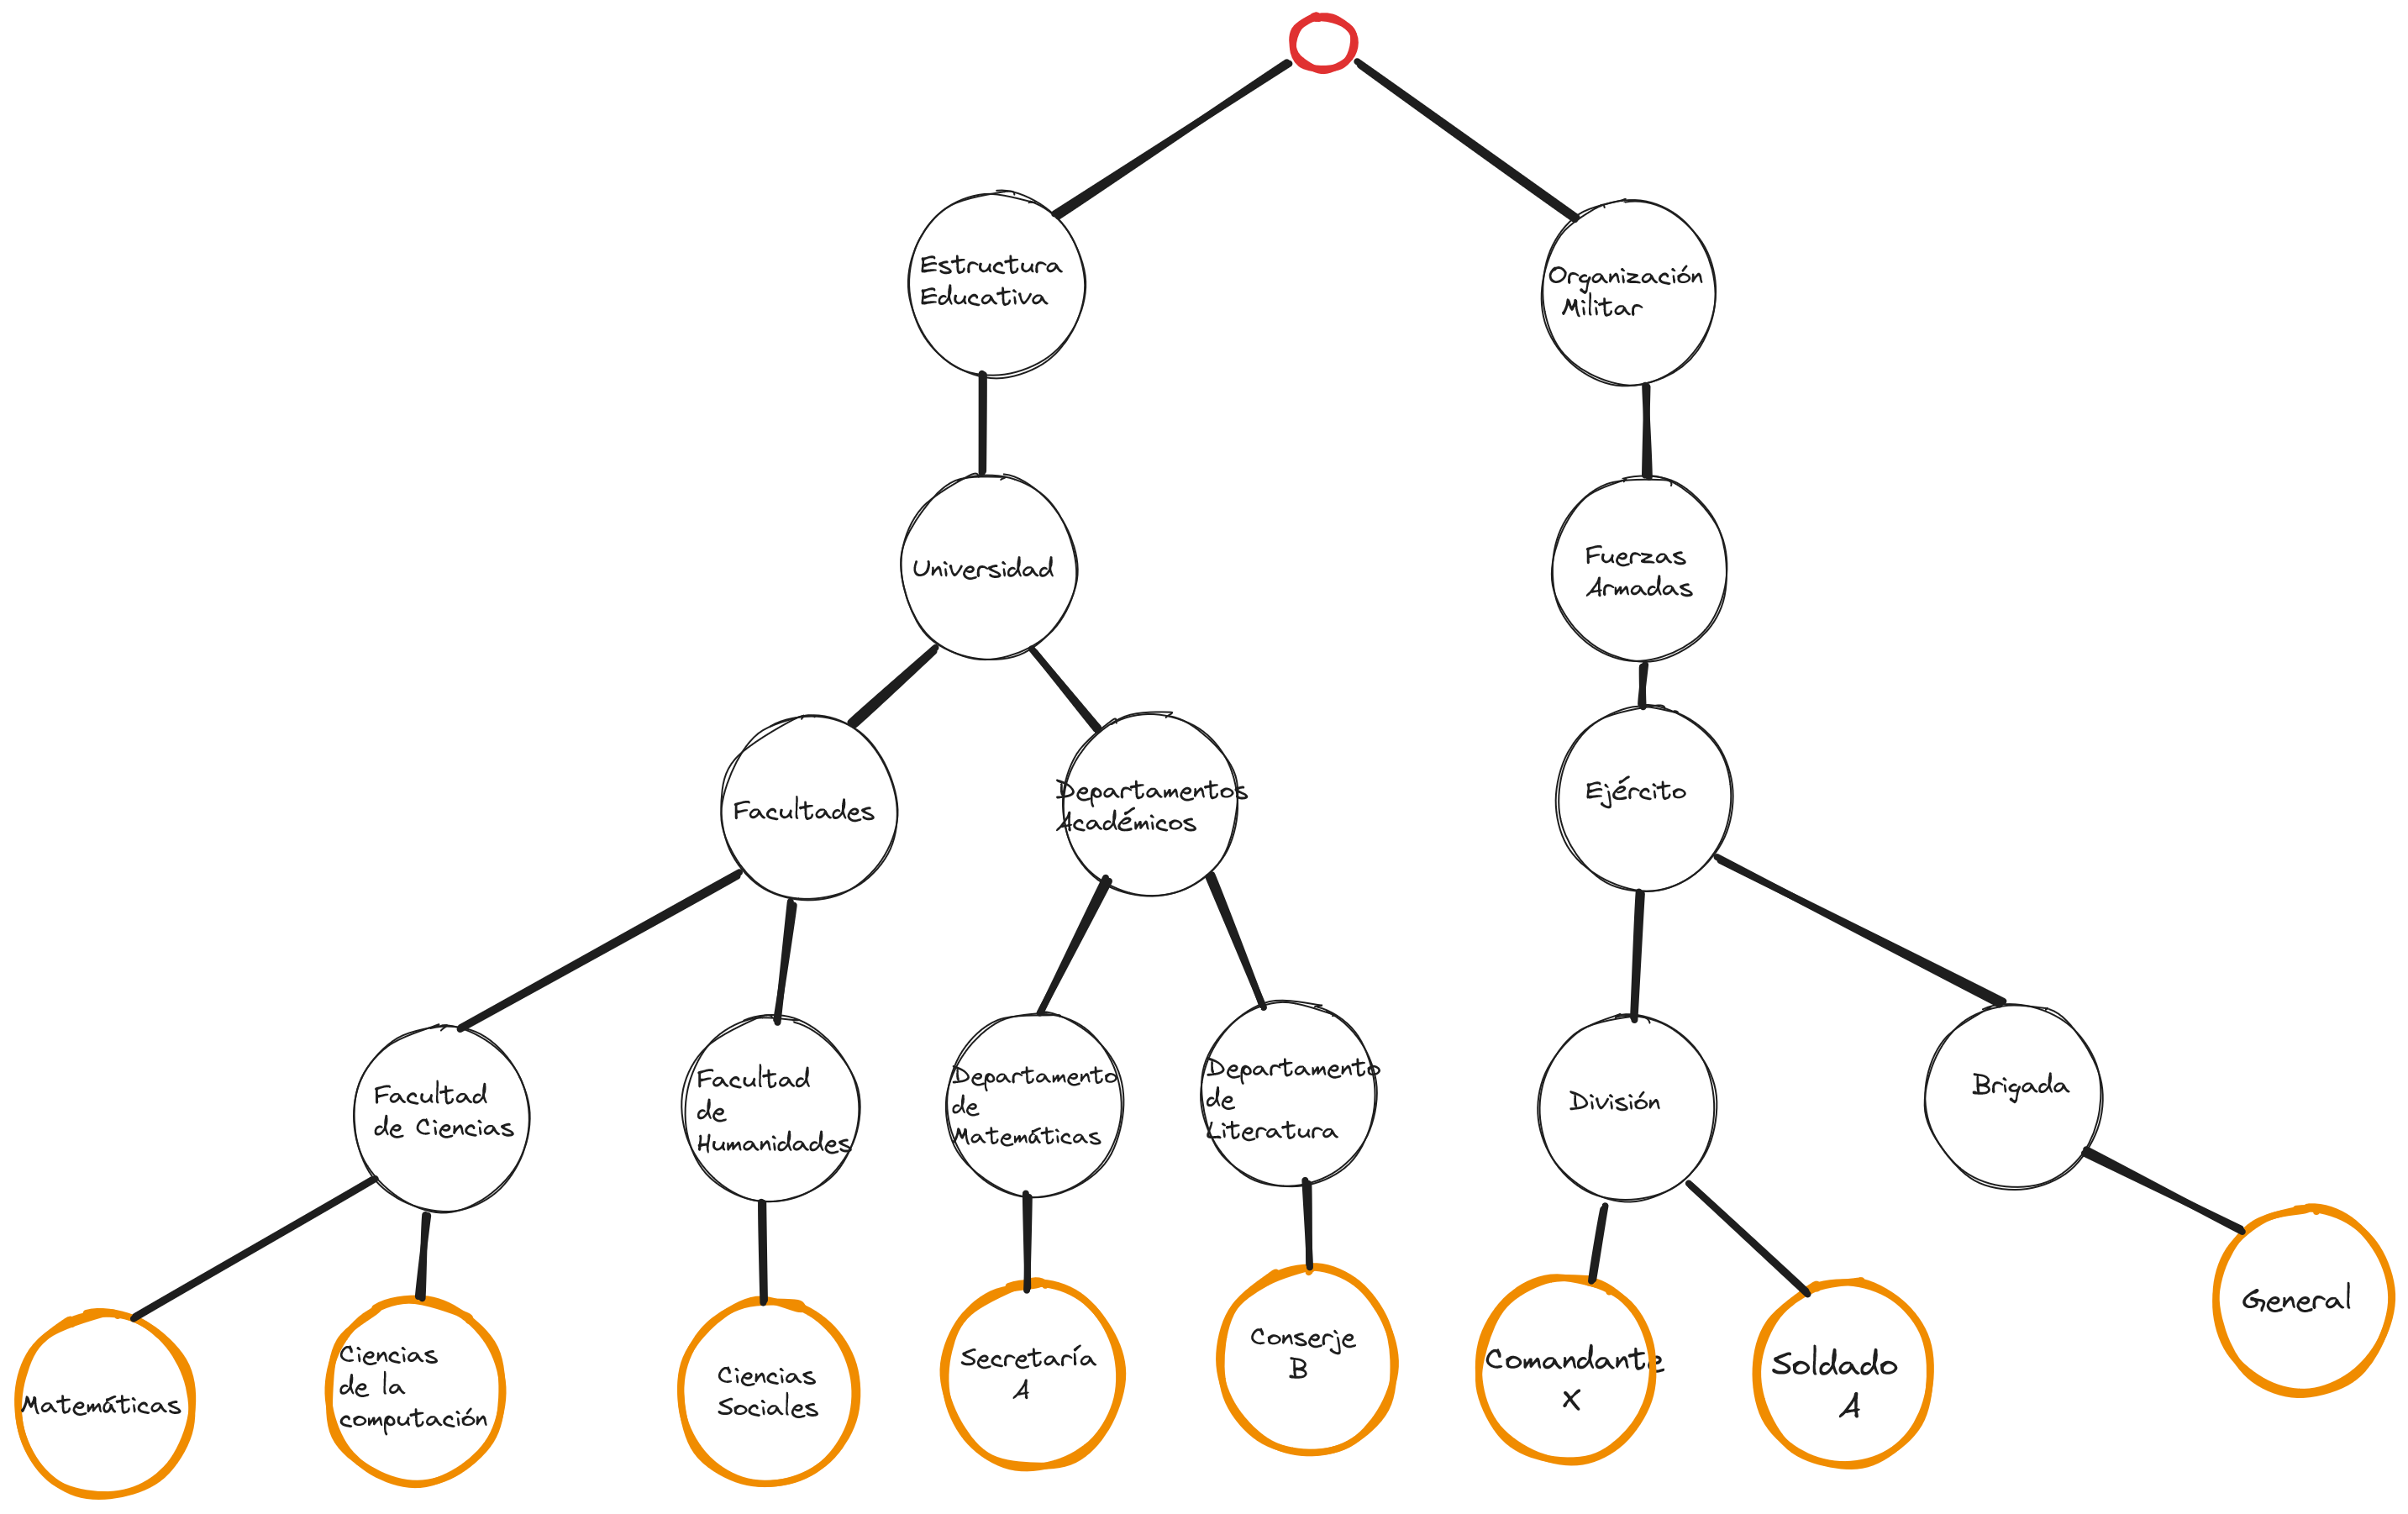
\includegraphics[scale=0.1]{../Image/Arbol.png}
\end{center}

No dibujó los números de cuenta en su diagrama para ahorrar espacio pero cada nodo tiene su número de cuenta. Ahora con ese árbol solo tiene que hacer un recorrido DFS hasta llegar a las hojas para obtener las cuentas de detalle y construir la tabla anterior.

El problema es que Urrutia olvido casi todo su conocimiento de su curso de estructuras de datos de segundo semestre, pero seguramente tu no, así que te pedimos que le ayudes a Urrutia dandole el algoritmo "Inserta" para construir este árbol N-ario, es decir cada nodo puede tener uno o varios hijos, consideraciones a tomar en cuenta es que el nodo raíz es un nodo maestro que no almacena información pero sostiene a los nodos que si la tienen.

Se espera usar tu algoritmo "Inserta" para ir insertando las filas de las tablas iniciales uno por uno en orden jerarquico en forma de nodos, los nodos almacenan los nombres de cuenta y las llaves se basan en los números cuenta separados por un guión pero no necesariamente tienen que ser exactamente iguales.

Hints: Observa como los números de cuenta son grupos separados por guiones, para pasar de un nivel de jerarquía mayor a uno menor se conserva el prefijo y se modifica el sufijo. \\ ¿Que pasaría si por ejemplo convertimos "1-00-00-00-0000" a "1" y "1-01-00-00-0000" a "1-1"? ¿Como sabemos que "1-1" es un número de cuenta de menor jerarquía que "1"? (2 puntos)\newline


$\rhd$\textbf{Solución.} \textit{Inserta}.
\begin{enumerate}
\item Tomemos a nuestra raíz como pivote y no insertemos valor alguno en ella.
\item Los dos hijos de la raíz serán $1$ y $2$, que son los posibles prefijos de las cuentas en ambas tablas.
\item Tenemos un formato X-Y-Z-... Entonces X debe ser $1$ o $2$, Y representará el siguiente nivel y será hijo
de X, luego Z representará un siguiente nivel y será hijo de Y, y así de manera sucesiva.
\item El árbol se comportará como un ``árbol ordenado'' bajo el siguiente criterio: si un nodo tiene 2 o más hijos estos
están dados de izquierda a derecha y de menor a mayor rango (i.e., insertamos 00 a la izquierda de 01 y a su vez 01
quedaría a la izquierda de 20). Así nuestro árbol guarda cierta jerarquía.
\end{enumerate}

¿Que pasaría si por ejemplo convertimos "1-00-00-00-0000" a "1" y "1-01-00-00-0000" a "1-1"? Iniciamos desde la raíz,
bajamos a $1$ (hijo izquierdo de la raíz) y seguimos bajando hacia la izquierda para encontrar "1-00-00-00-0000",
que tendrá una mayor jerarquía que "1-01-00-00-0000" por estar más a la izquierda en su recorrido hacia abajo.\newline

 ¿Como sabemos que "1-1" es un número de cuenta de menor jerarquía que "1"? Por el recorrido en profundidad, pues tenemos que
 movernos más a la derecha que para 1.
\hfill $\lhd$

\end{document}
